\section{Normale}
Modella variabili aleatorie continue che risultano dalla somma di molti effetti indipendenti e di piccola entità (teorema centrale del limite). 
È la distribuzione di riferimento in statistica e probabilità.

\[
\mathcal{N}(\mu,\sigma^2)
\]

\begin{figure}[H]
\centering

% ===================== PDF =====================
\begin{minipage}{0.45\textwidth}
\centering
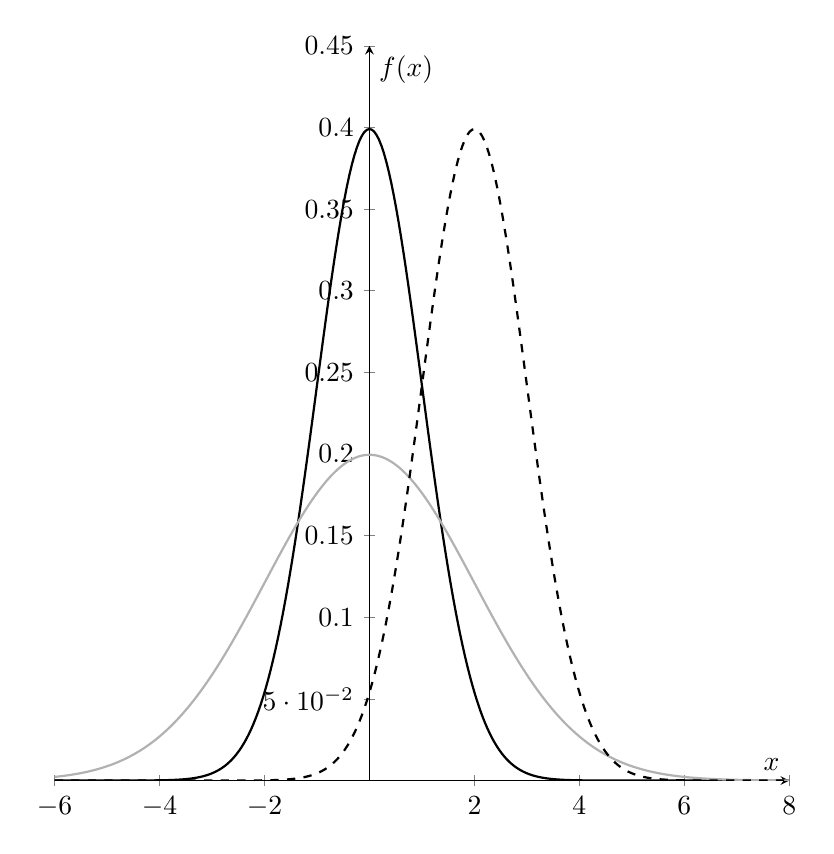
\begin{tikzpicture}
\begin{axis}[
    axis lines = middle,
    ylabel = {$f(x)$},
    xlabel = {$x$},
    width = 0.90\textwidth,
    height = 0.90\textwidth,
    ymin = 0, ymax = 0.45,
    xmin = -6, xmax = 8
]

% --- Normal(mu=0, sigma=1) ---
\addplot[black, thick, domain=-6:8, samples=300]
{1/sqrt(2*pi)*exp(-x^2/2)};

% --- Normal(mu=0, sigma=2) ---
\addplot[gray!60, thick, domain=-6:8, samples=300]
{1/(2*sqrt(2*pi))*exp(-x^2/8)};

% --- Normal(mu=2, sigma=1) ---
\addplot[dashed, thick, domain=-6:8, samples=300]
{1/sqrt(2*pi)*exp(-(x-2)^2/2)};

\end{axis}
\end{tikzpicture}
\end{minipage}
\hfill
% ===================== CDF =====================
\begin{minipage}{0.45\textwidth}
\centering

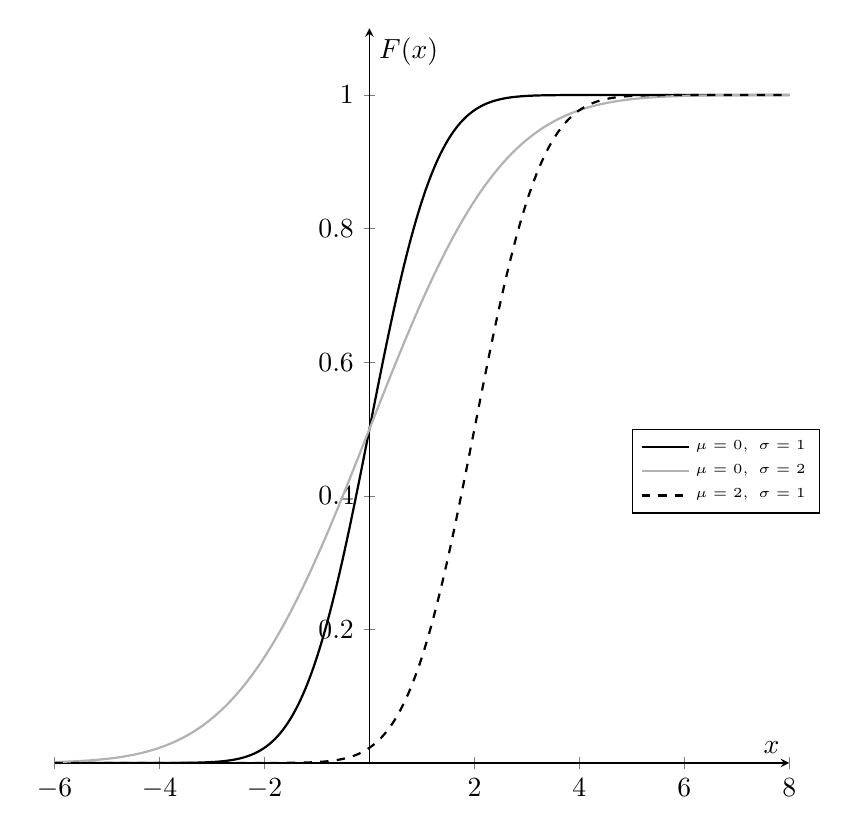
\begin{tikzpicture}[declare function={erf(\x)=%
    (1+(e^(-(\x*\x))*(-265.057+abs(\x)*(-135.065+abs(\x)%
    *(-59.646+(-6.84727-0.777889*abs(\x))*abs(\x)))))%
    /(3.05259+abs(\x))^5)*(\x>0?1:-1);}]

\begin{axis}[
    axis lines = middle,
    ylabel = {$F(x)$},
    xlabel = {$x$},
    width = 0.90\textwidth,
    height = 0.90\textwidth,
    ymin = 0, ymax = 1.1,
    xmin = -6, xmax = 8,
    legend style={at={(axis cs: 5,0.5)}, anchor=north west, font=\tiny},
    legend cell align=left,
]

% --- CDF Normal(mu=0, sigma=1) ---
\addplot[black, thick, domain=-6:8, samples=300]
{0.5*(1+erf(x/(1*sqrt(2))))};
\addlegendentry{$\mu=0,\ \sigma=1$}

% --- CDF Normal(mu=0, sigma=2) ---
\addplot[gray!60, thick, domain=-6:8, samples=300]
{0.5*(1+erf(x/(2*sqrt(2))))};
\addlegendentry{$\mu=0,\ \sigma=2$}

% --- CDF Normal(mu=2, sigma=1) ---
\addplot[dashed, thick, domain=-6:8, samples=300]
{0.5*(1+erf((x-2)/(1*sqrt(2))))};
\addlegendentry{$\mu=2,\ \sigma=1$}

\end{axis}
\end{tikzpicture}

\end{minipage}

\end{figure}

\bigskip
\begin{table}[H]
\centering
\renewcommand{\arraystretch}{2}
\begin{tabular}{@{}ll@{}}
\toprule
\textbf{Supporto} 
& $\mathbb{R}$ \\

\midrule

\textbf{Funzione di Densità} 
& $
f(x)=\dfrac{1}{\sqrt{2\pi\sigma^2}}
\ex{-\dfrac{(x-\mu)^2}{2\sigma^2}}
$ \\

\midrule

\textbf{Funzione di Ripartizione}
& $
F(x)= \Phi \left(\dfrac{t-\mu}{\sigma} \right) = \dfrac{1}{2}\left[1+\operatorname{erf}\!\left(\dfrac{x-\mu}{\sigma\sqrt{2}}\right)\right]
$ \\

\midrule

\textbf{Valore atteso} 
& $\mathbb{E}[X]=\mu$ \\

\midrule

\textbf{Varianza}
& $Var(X)=\sigma^2$ \\

\midrule

\textbf{Funzione caratteristica}
& $
\varphi_X(u)=
\ex{i\mu u - \frac{1}{2}\sigma^2 u^2}
$ \\

\bottomrule
\end{tabular}
\end{table}

